%%%%%%%%%%%%%%%%%%%%%%%%%%%%%%%%%%%%%%%%%%%%%%%%%%%%%
%												    %
%	PROTOCOLO LIGACAO DADOS						    %
%												    %
%	Novembro 2015								    %
%												    %
%	Angela Cardodo e Bruno Madeira					%
%   											    %	
%%%%%%%%%%%%%%%%%%%%%%%%%%%%%%%%%%%%%%%%%%%%%%%%%%%%%

\documentclass[11pt,a4paper,reqno]{report}
\linespread{1.2}


\usepackage{rotating}
\usepackage{tikz}
\usepackage[active]{srcltx}    
\usepackage{graphicx}
\usepackage{amsthm,amsfonts,amsmath,amssymb,indentfirst,mathrsfs,amscd}
\usepackage[mathscr]{eucal}
\usepackage{tensor}
\usepackage[utf8x]{inputenc}
\usepackage[portuges]{babel}
\usepackage[T1]{fontenc}
\usepackage{enumitem}
\setlist{nolistsep}
\usepackage{comment} 
\usepackage{tikz}
\usepackage[numbers,square, comma, sort&compress]{natbib}
\usepackage[nottoc,numbib]{tocbibind}
%\numberwithin{figure}{section}
\numberwithin{equation}{section}
\usepackage{scalefnt}
\usepackage[top=1cm, bottom=2cm, left=2cm, right=2cm]{geometry}
%\usepackage{tweaklist}
%\renewcommand{\itemhook}{\setlength{\topsep}{0pt}%
%	\setlength{\itemsep}{0pt}}
%\renewcommand{\enumhook}{\setlength{\topsep}{0pt}%
%	\setlength{\itemsep}{0pt}}
%\usepackage[colorlinks]{hyperref}
\usepackage{MnSymbol}
%\usepackage[pdfpagelabels,pagebackref,hypertexnames=true,plainpages=false,naturalnames]{hyperref}
\usepackage[naturalnames]{hyperref}
\usepackage{enumitem}
\usepackage{titling}
\newcommand{\subtitle}[1]{%
	\posttitle{%
	\par\end{center}
	\begin{center}\large#1\end{center}
	\vskip0.5em}%
}
\newcommand{\HRule}{\rule{\linewidth}{0.5mm}}
\usepackage{caption}
\usepackage{etoolbox}% http://ctan.org/pkg/etoolbox
\usepackage{complexity}

\usepackage[official]{eurosym}

\def\Cpp{C\raisebox{0.5ex}{\tiny\textbf{++}}}

\makeatletter
\def\@makechapterhead#1{%
  %%%%\vspace*{50\p@}% %%% removed!
  {\parindent \z@ \raggedright \normalfont
    \ifnum \c@secnumdepth >\m@ne
        \huge\bfseries \@chapapp\space \thechapter
        \par\nobreak
        \vskip 20\p@
    \fi
    \interlinepenalty\@M
    \Huge \bfseries #1\par\nobreak
    \vskip 40\p@
  }}
\def\@makeschapterhead#1{%
  %%%%%\vspace*{50\p@}% %%% removed!
  {\parindent \z@ \raggedright
    \normalfont
    \interlinepenalty\@M
    \Huge \bfseries  #1\par\nobreak
    \vskip 40\p@
  }}
\makeatother

\usepackage[toc,page]{appendix}

\addto\captionsportuges{%
  \renewcommand\appendixname{Anexo}
  \renewcommand\appendixpagename{Anexos}
}

\addto\captionsportuges{%
  \renewcommand\abstractname{\huge Sumário}  
}

\usepackage{verbatim}
\usepackage{color}
\definecolor{darkgray}{rgb}{0.41, 0.41, 0.41}
\definecolor{green}{rgb}{0.0, 0.5, 0.0}
\usepackage{listings}
\lstset{language=C++, 
    basicstyle=\linespread{0.8}\ttfamily,
    keywordstyle=\color{blue}\ttfamily,
	showstringspaces=false,
    stringstyle=\color{red}\ttfamily,
    commentstyle=\color{green}\ttfamily,
	identifierstyle=\color{darkgray}\ttfamily,
    morecomment=[l][\color{magenta}]{\#},
	tabsize=4,
    breaklines=true
}

\begin{document}



\begin{titlepage}
\begin{center}
 
\vspace*{3cm}

{\Large Redes de Computadores}\\[2cm]

% Title
{\Huge \bfseries Protocolo de Liga\c{c}\~ao de Dados \\[1cm]}

% Author
{\large \^Angela Cardoso e Bruno Madeira}\\[2cm]


\includegraphics[width=10cm]{feup_logo.jpg}\\[2cm]


% Bottom of the page
{\large \today}

\end{center}
\end{titlepage}


%%%%%%%%%%%
% SUMARIO %
%%%%%%%%%%%
\begin{abstract}
	
TODO: Parágrafo sobre contexto.
Relatório no âmbito da disciplina de Redes de Computadores relativo ao trabalho prático sobre Protocolos de Ligação e Dados.

TODO: Parágrafo sobre conclusões.

\end{abstract}

\tableofcontents


%%%%%%%%%%%%%%
% INTRODUCAO %
%%%%%%%%%%%%%%
\chapter{Introdução}

TODO: Indicação dos objectivos do trabalho e do relatório; descrição da lógica do relatório com indicações sobre o tipo de informação que poderá ser encontrada em cada uma secções seguintes.

Relatório relativo ao primeiro trabalho prático de Redes de Computadores que consiste na implementação de uma aplicação que transfere imagens entre dois computadores fazendo uso da porta-série. A aplicação deve usar um protocolo de ligação de dados \emph{Stop N Wait ARQ} híbrido que deve assegurar a fiabilidade  da transmissão mesmo em caso de desconexão. Deve também usar um protocolo de aplicação que é responsável pelo envio da imagem. O código desenvolvido deve ser estruturado em camadas, respeitando o princípio de encapsulamento, de modo a assegurar cada protocolo funciona de forma independente.
	
	O trabalho foi utilizando a linguagem de programação C num ambiente com um sistema operativo baseado em Linux. Para testes foi usada uma porta-seire XPTO???.
	
	Este relatório visa reportar qual o estado final da aplicação desenvolvia, clarificar detalhes do processo de implementação/código e a opinião dos estudantes face ao projecto realizado.
	
	Do capítulo 2 ao 4 são expostas as estruturas e os mecanismos implementados na concepção da aplicação sem incidir em detalhes específicos destes.
	Detalhes relativos à implementação dos protocolos são apresentados nos capítulos 5 e 6 e detalhes relativos à implementação de componntes extra são apresentados no capítulo 7.
	O capítulo 8 é relativo à validação e testes efectuados.
	
	
%%%%%%%%%%%%%%%
% ARQUITETURA %
%%%%%%%%%%%%%%%
\chapter{Arquitetura}

TODO:blocos funcionais e interfaces

diagrma de ..classes.. (os diversos moduos .h e ligações a dizer q este usa aquele ou alo semelhante)
blabla...
...no final
A \verb|utilities.h| foi criada com o intuito de ter métodos, estruturas e funcionalidades úteis a todos os módulos desenvolvidos. O seu uso principal no projecto é auxiliar o debug dos diversos modelos desenvolvidos.

%%%%%%%%%%%%%%%%%%%%
% ESTRUTURA CODIGO %
%%%%%%%%%%%%%%%%%%%%
\chapter{Estrutura do código}

%TODO: APIs, principais estruturas de dados, principais funções e sua relação com a arquitetura
Seguidamente são apresentadas as principais estruturas e funções desenvolvidas em cada módulo sendo algumas ocultadas uma vez que são referidas em maior detalhe nos capítulos relativos aos protocolos implementados.

\subsection{Estruturas de dados}
\begin{itemize}
\item \verb|applicationLayer|: declarada na \verb|App.c| contem informações básicas ao programa como o seu status (transmissor/receptor) por exemplo. 	
\item \verb|linkLayer|:declarada no \verb|DataLinkProtocol.c| serve para guardar as definições básicas da camada de ligação de dados como qual a porta série a ser usada.	
\item \verb|occurrences\_Log|:declarada no \verb|DataLinkProtocol.h| serve para registar ocorrências como o número de REJs recebidos.	
\end{itemize}

\subsection{Funções privadas da DataLinkProtocol}
\begin{itemize}
\item \verb|genBCC2| e \verb|validateBCC2| tratam respectivamente de gerar e de validar o BCC2.
\item \verb|write_UorS| e \verb|write_I| responsáveis pelo envio de tramas.
%getMessage e explicado no capitulo de protocolo
\item \verb|apply_stuffing| e \verb|apply_destuffing| realizam o stuffing e destuffing dos dados nas tramas I.
\item \verb|update_state_machine| função auxiliar que funciona como máquina de estados.
\item \verb|llopen_receiver|, \verb|llopen_transmitter|, \verb|llclose_receiver| e \verb|llclose_transmitter| ajudam a organizar o código do llopen e llclose uma vez que a sua execução difere do receptor para o emissor.
%\item \verb|timeout_alarm_handler|
\item \verb|startAlarm| e \verb|stopAlarm|
\end{itemize}

\subsection{Funções privadas da AppProtocol.c}
\begin{itemize}
\item \verb|receivePacket|
\item \verb|getControlPacket| e \verb|getInfoPacket|
\item \verb|sendControlPacket| e \verb|sendInfoPacket|
\item \verb|show_progress|
\end{itemize}

\subsection{Funções disponibilizadas por FileFuncs.h}
\begin{itemize}
\item \verb|getFileBytes| e \verb|save2File| são responsáveis respectivamente pela escrita e e leitura dos ficheiros.
\end{itemize}

%not impotant put only if it fits in a single page _>>>\subsection{Funções de user\_interface.c}

\subsection{Funções da App.c}
\begin{itemize}
%nao considerei o connect nem o setPacketSize mt importantes
\item \verb|receiveImage| e \verb|sendImage|
\item \verb|config|
\end{itemize}



%%%%%%%%%%%%%
% CASOS USO %
%%%%%%%%%%%%%
\chapter{Casos de uso principais}

TODO: identificação; sequências de chamada de funções
??? ??? ???
O diagrama de chamada de funções pode ser consultado no anexo \ref{flux}.

%%%%%%%%%%%%%%%%%%
% LIGACAO LOGICA %
%%%%%%%%%%%%%%%%%%
\chapter{Protocolo de ligação lógica}

Para implementar o protocolo de ligação lógica, seguimos as indicações do enunciado do projeto. Sendo assim, usamos a variante \emph{Stop and Wait}, o que significa que o Emissor, após cada mensagem, aguarda uma resposta do Recetor antes de enviar a mensagem seguinte. Isto significa, entre outras coisas, que podemos utilizar uma numeração módulo 2 para as mensagens, dado que nunca temos mais do que 2 mensagens em jogo (aquela que foi enviada e a que se pretende enviar de seguida).

O interface deste protocolo disponibiliza 6 funções. 

Quatro são as definidas pelo guião do trabalho (\verb|llopen|, \verb|llread|, \verb|llwrite|, \verb|llclose|) sendo que as únicas alterações efectuadas foram relativas à assinatura e funcionamento do \verb|llclose| de modo a permitir fechar a porta-série em caso de erro e no \verb|llopen|  que não recebe a porta a abrir. 

Estas 4 funções utilizam a função \verb|update_state_machine| para determinar a cada instante o estado em que está.
Com a concepção desta função evitou-se alguma repetição de código mas foi necessário cuidado extra na implementação pois são necessárias trocas de informação entre esta e a função que a invoca. A \verb|update_state_machine| recebe qual o tipo de trama esperada que serve para dentificar a função que a invocou e atualizar os estados corretamente e guarda numa variável auxiliar, \verb|received_C_type|, o tipo de trama recebida. Quando a função invocadora detecta que se atingio o estado \verb|STATE_MACHINE_STOP| verifica o \verb|received_C_type| para saber  tipo de trama recebido e como deve proceder.

Para obter a trama que se pretende enviar são usadas as funções \verb|write_UorS| e \verb|write_I| sendo estas respectivamente para o envio de tramas de Supervisão ou Não numeradas e para tramas de Informação. Elas fazem uso da função \verb|getMessage| que tem como parâmetros o Emissor original, o tipo e o número da trama e o array de caracteres onde será colocada a flag e o cabeçalho da trama. Posteriormente a estes bytes, em tramas de Informação, serão adicionados os dados e o respetivo BCC2. Nas restantes tramas, é apenas reutilizada a flag que está na primeira posição do array. A sua especificação pode ser encontrada no Anexo~\ref{tramas}.

As outras 2 funções disponibilizadas pelo interface são \verb|set_basic_definitions| e \verb|get_occurrences_log| que servem respectivamente para guardar as opções escolhidas pelo utilizador e para receber o registo de ocorrências na camada da aplicação.


%%%%%%%%%%%%%
% APLICACAO %
%%%%%%%%%%%%%
\chapter{Protocolo de aplicação}

O protocolo de aplicação foi implementado no ficheiro \verb|AppProtocol.c|. e apenas disponibiliza as funções \verb|sendFile| e \verb|receiveFile| para modulos externos. O protocolo foi implementado de acordo com o enunciado sendo que nos pacotes de controlo enviamos como parametros  nome e tamanho (em bytes) da imagem.

? ? ?

O envio/recepção de imagens atualiza uma variável, recebida por um apontador, externa ao Protocolo (definida num outro módulo), que indica os bytes já enviados/recebidos. Tal variável é usada atualmente dentro do protocolo para o display do estado de envio da imagem que inicialmente estava implementado no ficheiro \verb|user_interface.c|. Esta variável serviria também para tentar retransmitir uma imagem em caso de um envio falhar a meio. Este mecanismo de retransmissão não foi completado e o display foi movido pois o sua implementação inicial interferia com o envio/recepção de dados, a estrutura do código actual reflecte os planos inicialmente concebidos.

%%%%%%%%%%%%%%%
% VALORIZACAO %
%%%%%%%%%%%%%%%
\chapter{Elementos de valorização}

\section{Registo de ocorrências}

A camada de ligação de dados regista o número de tramas do tipo I e REJs recebidas/enviadas e o número de ocorrências de timeouts de uma transmissão. A informação fica registada numa variável do tipo \verb|occurrences_Log| e pode ser acedida pela componente de interface através do método \verb|get_occurrences_log|.

\section{Definições básicas}

O utilizador pode definir qual o \verb|baudrate| a usar, o \verb|packetSize| (numero de bytes máximos que envia da imagem em cada trama I antes de se realizar o stuffing) e o número máximo de tentativas consecutivas de reconexão.
Uma vez escolhidas as opções o intervalo de duração de um timeout é calculado em função do \verb|baudrate| e do \verb|packetSize| escolhidos pelo utilizador como se pode verificar no anexo \ref{setbasicdefinitions}. Na nossa implementação o receptor pode e deve configurar o \verb|baudrate| e \verb|packetSize| iguais aos do transmissor, pois, apesar de estes não serem usados na prática pelo receptor, são necessários para calcular um intervalo de timeout que seja fiável face às definições do transmissor.

\section{Gerador aleatório de erros e REJs}
São gerados erros aleatoriamente nas tramas enviadas pelo transmissor. São gerados erros no cabeçalho e de nos dados. Estes ocorrem de forma independente e são gerados respectivamente pelas funções \verb|randomErrorCabe| e \verb|randomErrorData|. A frequência destes erros é defina a partir das constantes \verb|CABE_PROB| e \verb|DATA_PROB| que representam quantas tramas são enviadas por cada um que apresenta um erro do tipo correspondente. Pode ser verificada a função \verb|randomErrorData| no anexo \ref{randomErrorData}. A \verb|randomErrorCabe| não foi incluída em anexo uma vez que é bastante semelhante à \verb|randomErrorData|.
Tramas do tipo REJ foram implementadas. Quando o receptor consegue identificar ocorrencia de erro(s) no bloco de dados envia uma mensagem ao transmissor e este trata de reenviar a pacote novamente.

\section{Representação do progresso}
Na AppProtocol.c, quando a aplicação está enviar/receber uma imagem, trata imprimir na consola a quantidade de bytes enviados/recebidos e quantos faltam para receber/enviar a imagem na totalidade. Este display (impressão na consola) é actualizado cada vez que um pacote é enviado/recebido na totalidade se já tiver passado um tempo mínimo definido na constante \verb|UPDATE_DISPLAY_MIN_TIME_INTERVAL| desde a ultima actualização de display de modo a evitar que ocorra com elevada frequência o que poderia tornar difícil a sua leitura ou afectar a

%%%%%%%%%%%%%
% VALIDACAO %
%%%%%%%%%%%%%
\chapter{Validação}

TODO: descrição dos testes efectuados com apresentação quantificada dos resultados, se possível

Foram realizados cerca de 10 testes ao longo das aulas práticas e fora destas usando uma porta-série.
Foram realizados cerca de 30 testes nas máquinas virtuais usadas para desenvolver a aplicação no fim desta estar terminada.
Relativamente à qualidade dos testes não foi usado nenhum auxiliar para verificar se as imagens recebidas eram iguais às enviadas nem nenhuma automatiação de testes, sendo estes todos realizados manualmente. 
Foram usadas imagens de diferentes tamanhos variados entre os 263 bytes (a mais pequena) e 712K bytes (a maior).Os tipos de imagens também variavam entre os tipos gif, jpeg e png.
De todos os testes realizados foram bem sucedidos à excepção de 1 que apresentou um aviso inesperado e do qual não conseguimos apurar o problema.

%%%%%%%%%%%%%%
% CONCLUSOES %
%%%%%%%%%%%%%%
\chapter{Conclusões}

Foi implementada com sucesso dentro do prazo establecido uma aplicação capaz de transferir imagens entre 2 computadores através de uma porta-série.
A implementação foi realizada em camadas como sugerido e foram percebidos os conceitos e implicações práticas dos protocolos usados.


%%%%%%%%%%%%%%%%
% BIBLIOGRAPHY %
%%%%%%%%%%%%%%%%
\bibliographystyle{IEEEtran}
\bibliography{rabb,refs}

\begin{appendices}

%%%%%%%%%%%%%%%%%%%%%%%%%%%
% APENDICE - CODIGO FONTE %
%%%%%%%%%%%%%%%%%%%%%%%%%%%
\chapter{Código Fonte}

\begin{lstlisting}
int llopen(app_status_type status)
{
	int fd;

	if (open_tio(&fd, 0, 0) != OK) {
		printf("\nERROR: Could not open terminal\n");
		return -1;
	}
	occ_log.num_of_Is = 0;
	occ_log.total_num_of_timeouts= 0;
	occ_log.num_of_REJs			 = 0;
	if (status == APP_STATUS_TRANSMITTER)
	{
		app_status = APP_STATUS_TRANSMITTER;
		if( llopen_transmitter(fd) != OK) {
			close_tio(fd);
			return -1;
		};
	}
	else if (status == APP_STATUS_RECEIVER)
	{
		app_status = APP_STATUS_RECEIVER;
		if( llopen_receiver(fd) != OK) {
			close_tio(fd);
			return -1;
		};
	}
	else
	{
		printf("\nWARNING(llo):invalid app_status found on llopen().\n");
		close_tio(fd);
		return 1;
	}
	return fd;
}
\end{lstlisting}

\section{Função set\_basic\_definitions em DataLinkProtocol.c}
\label{setbasicdefinitions}
\begin{lstlisting}
void set_basic_definitions(int number_of_tries_when_failing, char* port, int baudrate, int packetSize)
{
	DEBUG_SECTION(DEBUG_PRINT_SECTION_NUM,
		printf("\n-section1-");
	sleep(1);
	);

	signal(SIGALRM, timeout_alarm_handler);
	
	int realbauds[20] = {0, 50, 75, 110, 134, 150, 200, 300, 600, 1200, 1800, 2400, 4800, 9600, 19200, 38400, 57600, 115200, 230400, 460800};
	int realBaudrate;
	if (baudrate <= 15) realBaudrate = realbauds[baudrate];
	else realBaudrate = realbauds[baudrate - 4081];
	
	int timeout_in_seconds = ((packetSize + 4 + 1) * 2 + 5) / (realBaudrate / 8) + 1;
	printf("size: %d\n", packetSize);
	printf("baudrate: %d\n", realBaudrate);
	printf("timeout: %d\n", timeout_in_seconds);
	link_layer_data.timeout = timeout_in_seconds;
	link_layer_data.numTransmissions = number_of_tries_when_failing;
	if (port_name_was_set == NO) { strcpy(link_layer_data.port, port); port_name_was_set = YES; }
	link_layer_data.baudRate = baudrate;
}
\end{lstlisting}

%-------------------------------------------------------------------------------------------------------------------------------------------------
\section{Função randomErrorData em DataLinkProtocol.c }
\label{randomErrorData}
\begin{lstlisting}
void randomErrorData(char* trama, int data_size) {	
	int trama_byte;
	if (DATA_PROB > 0) {
		int data_error = rand() % DATA_PROB;
		if (data_error == 0) {
			trama_byte = rand() % data_size;	// escolher o byte de erro na zona dos dados da trama
			trama[trama_byte]++;			// o erro e incrementar o byte escolhido
		}
	}
}
\end{lstlisting}
%-------------------------------------------------------------------------------------------------------------------------------------------------




\chapter{Tipos de Tramas Usadas}
\label{tramas}

As tramas que utilizamos podem ser de três tipos:
\begin{itemize}
	\item Informação (I) - transportam dados;
	\item Supervisão (S) - são usadas para iniciar e terminar a transmissão, assim como para responder a tramas do tipo I;
	\item Não Numeradas (U) - são usadas para responder a tramas de início e fim de transmissão.
\end{itemize}

Todas as tramas são delimitadas pelas \emph{Flags} F - 01111110. Além disso, independentemente do tipo da trama, o cabeçalho é sempre o mesmo conjunto de 3 bytes:
\begin{enumerate}
	\item A - Campo de Endereço - 00000011 em comandos enviados pelo Emissor e respostas enviadas pelo Receptor, 00000001 na situação inversa;
	\item C - Campo de Controlo:
		\begin{itemize}
			\item tramas I - 00S00000, onde S é o bit que identifica a trama;
			\item tramas SET (\emph{set up}) - 00000111;
			\item tramas DISC (\emph{disconnect})- 00001011;
			\item tramas UA (\emph{unnumbered acknowledgment}) - 00000011;
			\item tramas RR (\emph{positive acknowledgment}) - 00R00001, onde R identifica a trama;
			\item tramas REJ (\emph{negative acknowledgment}) - 00R00101, onde R identifica a trama;
		\end{itemize}
	\item BCC1 (\emph{Block Check Character}) - Campo de Proteção do Cabeçalho - é obtido realizando a disjunção exclusiva bit a bit de A e C.
\end{enumerate} 

Se se tratar de uma trama I, após o cabeçalho temos:
\begin{itemize}
	\item $\text{D}_{\text{1}}, \text{D}_{\text{2}}, \ldots, \text{D}_{\text{N}}$ - bytes de dados;
	\item BCC2 - Campo de Proteção dos Dados - calculado de forma que exista um número par de 1s em cada bit dos dados, incluindo o BCC2.
\end{itemize}

As restantes tramas apenas têm o respetivo cabeçalho delimitado por flags.

%--------------------------------------------------------------------------------------------------------------------------------------------

\chapter{Diagrama de chamadas a funções (Fluxo)}
\label{flux}
\begin{sidewaysfigure}
\centering
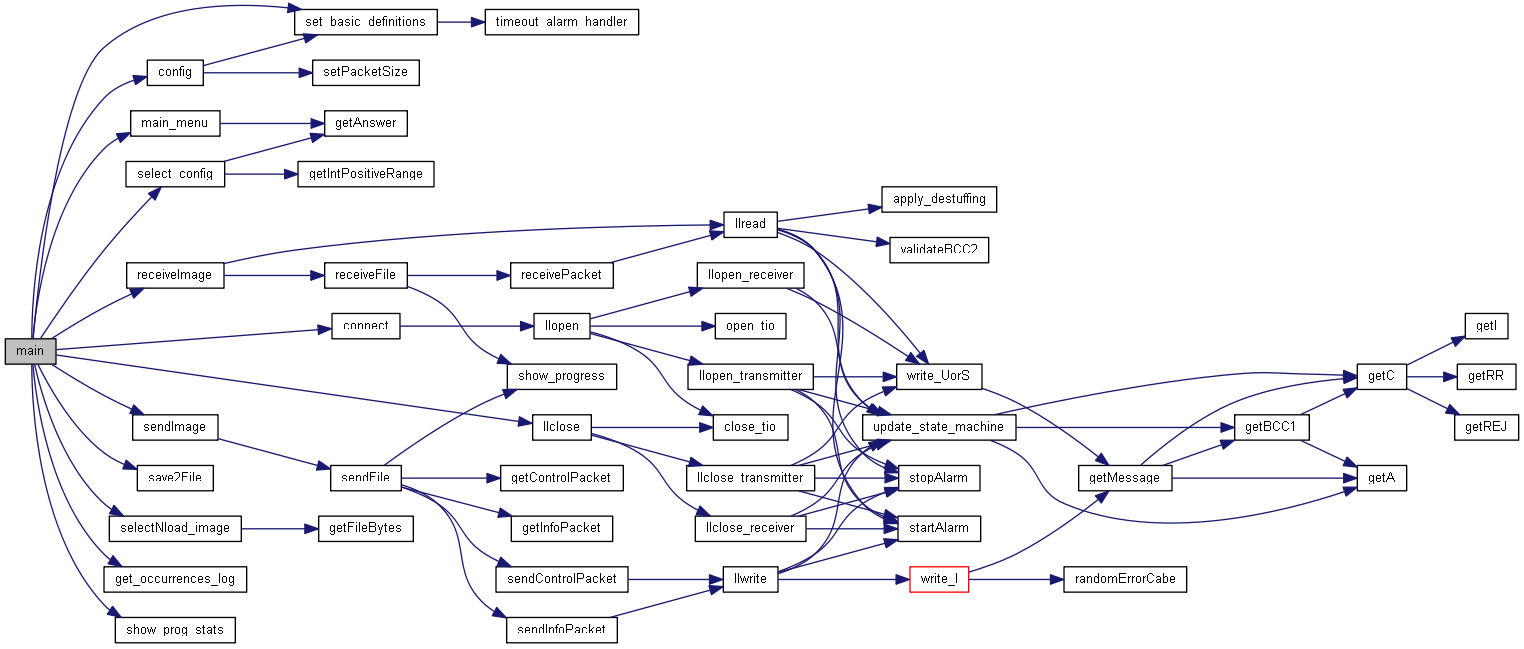
\includegraphics[width=26cm]{_app_8c_a3c04138a5bfe5d72780bb7e82a18e627_cgraph.png}
\end{sidewaysfigure}

%---------------------------------------------------------------------------------------------------------------------------------------------

\chapter{Diagrama de chamadas a funções (Fluxo)}
\label{modulediagram}
\centering
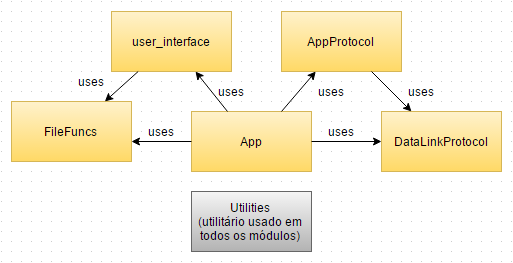
\includegraphics[width=15cm]{rcom_module_diagram.png}

\end{appendices}

\end{document}
